\documentclass[a4paper, DIV12, 2.5headlines, bigheadings, titlepage, openbib]{scrartcl}

\usepackage[ngerman, english]{babel}
\usepackage[T1]{fontenc}
\usepackage{geometry}
\usepackage[utf8x]{inputenc}
\usepackage{mathpazo}
\usepackage{helvet}
\usepackage{courier}
\usepackage{eurosym}
\usepackage{amsmath}
\usepackage{courier}
\usepackage{scrpage2}
\usepackage{graphicx}
\usepackage{xcolor}
\usepackage{multirow}
\usepackage{varioref}
\usepackage{babelbib}
\usepackage{makeidx}
\usepackage{tabularx}
\usepackage{floatflt}
\usepackage{float}
\usepackage{lipsum}
\usepackage{xargs}
\usepackage{enumitem}
\usepackage{listings}
\usepackage[colorinlistoftodos,prependcaption,textsize=tiny]{todonotes}
\usepackage[pdftex, colorlinks, linktocpage, linkcolor=black, citecolor=black, urlcolor=black]{hyperref}
\usepackage[linesnumbered]{algorithm2e}
\setlength\abovecaptionskip{-15pt}

\pagestyle{scrheadings}

\geometry{a4paper, top=55mm, left=40mm, right=35mm, bottom=40mm, headsep=10mm, footskip=22mm}
\linespread {1.25}

\newcommand{\theauthor}{Stephan Schultz}
\newcommand{\matrnr}{766872}
\newcommand{\thetitle}{Accessing and transferring sensor data on Wearables in real-time}
\newcommand{\thesubtitle}{Zugriff und Übertragung von Sensor Daten auf Wearables in Echtzeit}

\definecolor{code_background}{HTML}{FFFFFF}
\definecolor{code_comments}{HTML}{969896}
\definecolor{code_keywords}{HTML}{A71D5D}
\definecolor{code_numbers}{HTML}{969896}
\definecolor{code_strings}{HTML}{183691}
\definecolor{code_identifiers}{HTML}{444444}
% Rot
\definecolor{hpired}{rgb}{0.686,0,0.204}
% Orange
\definecolor{hpiorange}{rgb}{0.867,0.380,0.031}	
% Gelb
\definecolor{hpiyellow}{rgb}{0.965,0.659,0}					%100 
\colorlet{hpiyellow2}{hpiyellow!60!white}					% 60
\colorlet{hpiyellow3}{hpiyellow!40!white}					% 40
\colorlet{hpiyellow4}{hpiyellow!20!white}					% 20
% Grau
\definecolor{hpigrey}{rgb}{0.376,0.408,0.420}				%100
\colorlet{hpigrey2}{hpigrey!70!white}						% 70
\colorlet{hpigrey3}{hpigrey!50!white}						% 50
\colorlet{hpigrey4}{hpigrey!20!white}						% 20
% Blau
\definecolor{hpiblue}{rgb}{0,0.478,0.620}					%100
\colorlet{hpiblue2}{hpiblue!60!white}						% 60
\colorlet{hpiblue3}{hpiblue!40!white}						% 40
\colorlet{hpiblue4}{hpiblue!15!white}						% 15
\usepackage{array}
\usepackage{supertabular}
\usepackage{colortbl}

\newcounter{todocounter}
\setcounter{todocounter}{0}
\newcounter{authcounter}
\setcounter{authcounter}{0}
%%% BEGIN Write TODO in File
\def\getdefhelp#1->#2\endhelp{#2}
\def\getdef#1#2{\edef#2{\expandafter\getdefhelp\meaning#1\endhelp}}
\newwrite\TodoDatei
\newwrite\AuthorDatei
\openout\AuthorDatei=author.out
\newcommand{\WriteTodo}[2]{%
	\def\Cont{#2}
	\getdef\Cont\Content
	\edef\WriteIndex{%
		\write\TodoDatei{\string\textcolor{#1}{\string\textbf{\Content}}\string\dotfill\string\pageref{todo:\thetodocounter}}}%
	\WriteIndex}

\newcommand{\WriteAuthor}[1]{%
	\def\Cont{#1}
	\getdef\Cont\Content
	\edef\WriteAuth{\write\AuthorDatei{\Content\string\dotfill\string\ref{auth:\theauthcounter}}}
	\WriteAuth}


%%% END Write TODO in File

% command \BibTeX
\def\BibTeX{{\rm B\kern-.05em{\sc i\kern-.025em b}\kern-.08em
     T\kern-.1667em\lower.7ex\hbox{E}\kern-.125emX}} 

% day in journal: \journalday{date}{titel}{persons}{aktivity}
\newcommand{\journalday}[4]{%
\def\titleTmp{#2}
\subsection*{#1\ifx\titleTmp\empty{}\else{: #2}\fi}
\begin{center}
\begin{tabularx}{\textwidth}{@{}lX@{}}
	Anwesende: & #3\\
	Vorgang: & #4
\end{tabularx}
\end{center}
}

% errorreport: \errorreport{date}{error}{reason}{solution}
\newcommand{\errorreport}[4]{%
\def\dateTmp{#1}
\def\errorTmp{#2}
\def\reasonTmp{#3}
\def\solutionTmp{#4}
\ifx\errorTmp\empty{}\else{%
\subsection*{\ifx\dateTmp\empty{}\else{\hfill(#1)\\}\fi Problem: #2}%
{\begin{center}%
\vskip-1ex%
\begin{tabularx}{\linewidth}{@{}lX@{}}
	Ursache: & \ifx\reasonTmp\empty{unbekannt}\else{#3}\fi\\
	L�sung: & \ifx\solutionTmp\empty{unbekannt}\else{#4}\fi\\
\end{tabularx}%
\end{center}%
}}\fi}

% code: \code[textcolor]{backgroundcolor}{content}
\newcommand{\code}[3][black]{%
	\begin{flushleft}	
		\ttfamily
		\small
		\fcolorbox{#1}{#2}{\textcolor{#1}{\shortstack[l]{#3}}}
	\end{flushleft}
}

% code with white borderline
\newcommand{\codeblank}[3][black]{%
	\begin{flushleft}	
		\ttfamily
		\small
		\fcolorbox{white}{#2}{\textcolor{#1}{\shortstack[l]{#3}}}
	\end{flushleft}
}

% centered code: \centercode[textcolor]{backgroundcolor}{content}
\newcommand{\centercode}[3][black]{%
	\begin{center}	
		\ttfamily
		\small
		\fcolorbox{#1}{#2}{\textcolor{#1}{\shortstack[l]{#3}}}
	\end{center}
}

% centered code with white borderline
\newcommand{\centercodeblank}[3][black]{%
	\begin{center}	
		\ttfamily
		\small
		\fcolorbox{white}{#2}{\textcolor{#1}{\shortstack[l]{#3}}}
	\end{center}
}


% annotation in colored box: \annot[text- and bordercolor]{backgroudcolor}{contents}
\newcommand{\annot}[3][black]{%
	\begin{center}	
		\fcolorbox{#1}{#2}{\textcolor{#1}{\shortstack[l]{\vspace*{1ex}\\\hspace*{.025\textwidth}\textbf{Anmerkung:}\\\hspace*{.05\textwidth}\parbox{.88\textwidth}{#3\vspace*{2ex}}\hspace*{.05\textwidth}}}}
	\end{center}
}

% annotation in colored box: \annot[text- and bordercolor]{backgroudcolor}{contents}
\newcommand{\hint}[3][black]{%
\begin{figure}[!t]
  \centering
  \fcolorbox{#1}{#2}{
    \begin{minipage}{.96\linewidth}
      \hspace*{.025\linewidth}\parbox{.93\linewidth}{\textbf{Hinweis:}}\hspace*{.025\linewidth}\\
      \hspace*{.05\linewidth }\parbox{.88\linewidth}{\vspace*{3ex}#3\vspace*{3ex}}\hspace*{.05\linewidth}
    \end{minipage}
  }
\end{figure}
}

\newcommand{\colorparbox}[3][.985\textwidth]{%
\begin{flushleft}
\fcolorbox{black}{#2}{\parbox{#1}{#3}}
\end{flushleft}
}

\newcounter{versionID}
\newenvironment{versioning}[1][hpiblue4]{%
\setcounter{versionID}{0}
\begin{center}	
	\tablefirsthead{%
		\hline
		\rowcolor{#1}
		\parbox[c][2em][c]{\linewidth}{\centering\textbf{lfd. Nr.}} &
		\parbox[c][2em][c]{\linewidth}{\centering\textbf{Bearbeiter}} & 
		\parbox[c][2em][c]{\linewidth}{\centering\textbf{�nderungen}}\\
		\hline}
	\tablehead{%
		\extrahead
		\hline
		\rowcolor{#1}
		\parbox[c][2em][c]{\linewidth}{\centering\textbf{lfd. Nr.}} &
		\parbox[c][2em][c]{\linewidth}{\centering\textbf{Bearbeiter}} & 
		\parbox[c][2em][c]{\linewidth}{\centering\textbf{�nderungen}}\\
		\hline}
	\tabletail{%
		\hline
		\multicolumn{3}{|r|}{\cellcolor{hpiblue4}\small\sl Fortsetzung auf der n�chsten Seite}\\
		\hline}
	\tablelasttail{}
	\begin{supertabular}{|p{.1\linewidth}|p{.25\linewidth}|p{.5\linewidth}|}
	}{%
	\end{supertabular}
\end{center}
\newwrite\VersionDatei
\openout\VersionDatei=theversion.aux
\write\VersionDatei{\theversionID}
\closeout\VersionDatei
%\vfill
}

\newcommand{\version}[2]{%
\parbox{\linewidth}{\centering\stepcounter{versionID}\theversionID} & 
\parbox[t]{\linewidth}{\centering#1} &
#2 \\\hline
}

\newcommand{\currentversion}[1][]{
\def\test{#1}
\def\drafttest{draft}
\def\finaltest{final}
\ifx\test\drafttest
	\def\versiontext{(Entwurf)}
\else
	\ifx\test\finaltest
		\def\versiontext{(Final)}
	\else
		\def\versiontext{}
	\fi
\fi
\vskip.3cm
\newread\DatenDatei
\openin\DatenDatei=theversion.aux
\ifeof\DatenDatei\def\curVers{---}\else\read\DatenDatei to \curVers\fi
\closein\DatenDatei
{\small Dokumentversion: \curVers{}\versiontext}}

%% Acceptance Criterions
\newenvironment{acceptance}[1][hpiblue4]{%
\begin{center}	
	\tablefirsthead{%
		\hline
		\multicolumn{2}{|l|}{\cellcolor{hpiblue3}\bfseries Abnahmekriterien:}\\
		\hline}
	\tablehead{%
		\hline
		\multicolumn{2}{|l|}{\cellcolor{hpiblue3}\bfseries Abnahmekriterien (Fortsetzung):}\\
		\hline}
	\tabletail{%
		\multicolumn{2}{|r|}{\cellcolor{hpiblue4}\small\sl Fortsetzung auf der n�chsten Seite}\\
		\hline}
	\tablelasttail{}
	\begin{supertabular}{p{.23\linewidth}p{.7\linewidth}}
	}{%
	\end{supertabular}
\end{center}
\vfill
}

\newcommand{\criterion}[3]{%
	& \\
	\rowcolor{hpiblue4}Ausgangssitiation: & #1 \\
	Ereignis: & #2 \\
	Erwartetes Ergebnis: & #3 \\
}

\newcommand{\authindex}[1]{\expandafter\index{#1}}
%% SecAuthor
\newcommand{\secauthor}[2]{%
\def\secChap{chapter}
\def\secSect{section}
\def\secSubs{subsection}
\edef\refer{#1!Abschnitt \thesection}
\def\sec{#2}
\ifx\sec\secChap\edef\refer{#1!Kapitel \thechapter}\fi
\ifx\sec\secSect\edef\refer{#1!Abschnitt \thesection}\fi
\ifx\sec\secSubs\edef\refer{#1!Abschnitt \thesubsection}\fi
\label{auth:\theauthcounter}
\authindex{\refer}
%In Datei schreiben
%\WriteAuthor{#2}
\stepcounter{authcounter}
}

%% Todo
\newcommand{\todo}[2][normal]{%
\def\test{#1}
\def\hightest{high}
\def\lowtest{low}
%\def\normaltest{normal}
\ifx\test\hightest
	\def\prioritycolor{hpired}
\else
	\ifx\test\lowtest
		\def\prioritycolor{hpiyellow}
	\else
		\def\prioritycolor{hpiorange}
	\fi
\fi
\par{\raggedright
	\color{\prioritycolor}TODO: #2
	\label{todo:\thetodocounter}
	\WriteTodo{\prioritycolor}{#2}
	\stepcounter{todocounter}
}\par
}

\newif\ifnotdone

\newcommand{\readLine}[1]{%
\ifeof#1
	\def\tobedone{}
	\notdonefalse
\else
	\read\TodoFileIn to \tobedone
	\notdonetrue
\fi
\tobedone\par}

\newcommand{\listtodo}{%
\begin{flushleft}
	\newread\TodoFileIn
	\openin\TodoFileIn=todo.out
	\loop
		\readLine{\TodoFileIn}
	\ifnotdone
	\repeat
	\closein\TodoFileIn
	\immediate\openout\TodoDatei=todo.out
\end{flushleft}
}

%%% XML-Command
\newdimen\LineFeedDim
\LineFeedDim = 1.5em
\newdimen\LineFeed
\newif\ifXMLintern

\newcommand{\Tag}[4][black]{%
\ifXMLintern\\\hskip\LineFeed\fi%
\XMLinternfalse%
\textcolor{#1}{<#2}%
\def\paratest{#3}%
\ifx\paratest\empty{}%
\else{} #3%
\fi%
\global\advance\LineFeed by \LineFeedDim%
\def\contenttest{#4}%
\ifx\contenttest\empty%
	\global\advance\LineFeed by -\LineFeedDim\textcolor{#1}{/>}%
\else%
\textcolor{#1}{>}\\\hskip\LineFeed#4\\%
\global\advance\LineFeed by -\LineFeedDim\ifdim\LineFeed > 0em\hskip\LineFeed\fi\textcolor{#1}{</#2>}%
\fi\XMLinterntrue%
}

%% <? ... ?> als Argument �bergeben -> processing, comment, normal
\def\proctest{processing}
\def\commtest{comment}
\def\normtest{normal}
\newcommand{\LineTag}[4][normal]{%
\ifXMLintern\\\hskip\LineFeed\fi%
\XMLinternfalse%
\def\argtest{#1}%
<\ifx\argtest\proctest ?\else\ifx\argtest\commtest !-- \fi\fi#2%
\def\partest{#3}%
\ifx\partest\empty%
\else{} %
	#3%
\fi%
\def\contenttest{#4}%
\ifx\contenttest\empty%
\def\argtest{#1}%
\ifx\argtest\proctest{} ?\else\ifx\argtest\commtest{} --\else/\fi\fi>%
\else> #4 </#2>\fi\XMLinterntrue%
}

\newcommand{\EmptyTag}[1][]{%
\ifXMLintern\\\hskip\LineFeed\fi#1\parbox[c][1ex][c]{1ex}{}\XMLinterntrue%
}

\newcommand{\NewLinePar}{%
\\\hskip\LineFeed\hskip3em
}

\newcommand{\xml}[3][black]{%
	\LineFeed=0em
	\XMLinternfalse
	\small
	\fcolorbox{#1}{#2}{\ttfamily\shortstack[l]{#3}}
}

\newcommand{\soapmsg}[7][hpigray4]{%
	{\centering
	\begin{tabularx}{\linewidth}{|l|X|}
		\hline
		\cellcolor{#1}K�rzel & #2 \\
		\hline
		\cellcolor{#1}Consumer & #3 \\
		\hline
		\cellcolor{#1}Request Parameter & #4 \\
		\hline
		\cellcolor{#1}Response Parameter & #5 \\
		\hline
		\cellcolor{#1}Kurzbeschreibung & #6 \\
		\hline%
		\cellcolor{#1}Doppelter Request & #7 \\
		\hline
	\end{tabularx}
	}
}

\newcommand{\myabstract}[2]{%
	\def\germtest{#1}
	\def\engltest{#2}
	\ifx\germtest\empty
		\ifx\engltest\empty
		\else
			\hbox{ }
			\vfill
		\fi
	\else
		\hbox{ }
		\vfill
  \fi
	\ifx\germtest\empty\else
  	\begin{quotation}
  	\begin{center}\normalfont\sectfont\nobreak Kurzfassung\end{center}
  	#1
  	\end{quotation}
  	\vskip1cm
  \fi
  \ifx\engltest\empty\else
  	\begin{quotation}
  	\begin{center}\normalfont\sectfont\nobreak Abstract\end{center}
  	#2
  	\end{quotation}
	\fi
	\ifx\germtest\empty
		\ifx\engltest\empty
		\else
  		\vfill
  		\vfill
  		\clearpage
		\fi
	\else
  	\vfill
  	\vfill
  	\clearpage
  \fi
}
% Eigene Umgebungen
\newenvironment{otherenumi}[1]{%
	\renewcommand*{\labelenumi}{#1}
	\begin{enumerate}
	}{%
	\end{enumerate}
	\renewcommand*{\labelenumi}{\alph{enumi})}}
\newenvironment{otherenumii}[1]{%
	\renewcommand*{\labelenumii}{#1}
	\begin{enumerate}
	}{%
	\end{enumerate}
	\renewcommand*{\labelenumi}{\alph{enumi})}}


\lstdefinestyle{javastyle}{
    language=Java,
    backgroundcolor=\color{code_background},
    commentstyle=\color{code_comments},
    keywordstyle=\color{code_keywords},
    numberstyle=\tiny\color{code_numbers},
    stringstyle=\color{code_strings},
    identifierstyle=\color{code_identifiers},
    basicstyle=\scriptsize,
    xleftmargin=-20mm,
    xrightmargin=-30mm,
    breakatwhitespace=false,
    breaklines=true,
    captionpos=b,
    keepspaces=true,
    numbers=left,
    numbersep=5pt,
    showspaces=false,
    showstringspaces=false,
    showtabs=false,
    tabsize=2
}
\lstset{style=javastyle}

\setlength{\parindent}{0cm}
\setlength{\parskip}{0.25cm}

\begin{document}

	%%% Headers & Footers
	\selectlanguage{english}
	\automark{section}
	\ohead{
\includegraphics[height=1.3cm,clip,viewport={0 60 250 180}]{utils/hpi_logo.pdf}}
	\chead{}
	\ihead{\headmark}
	\setheadsepline{1.0pt}[\color{hpigrey}]

	%%% Title page
	\hypersetup{%
		pdftitle	= {\thetitle},
		pdfsubject	= {Bachelor Thesis},
		pdfauthor	= {\theauthor},
		pdfcreator	= {PDFLaTeX},
		pdfproducer	= {LaTeX with hyperref and thumbpdf}
	}
	
		\titlehead{
	%\parbox[b]{10cm}{\sffamily{\Large Hasso Plattner Institut}  \\Prof.~Dr.~Helmertstra�e~2-3 \\14482 Potsdam} 
	\centering
	
\includegraphics[height=4cm]{utils/hpi_logo_text.pdf}
	
	}		\subject{{\LARGE Bachelor's Thesis}\\}
	\title{\thetitle}
	\subtitle{\thesubtitle}
	\author{{\small by}\\\textbf{\theauthor}}
	%\dedication{Widmung\\mit mehreren\\Zeilen.}
	\date{Potsdam, July 2015}
	\publishers{
		\textbf{Supervisor}\\
		\vskip1em
		Prof. Dr. Christoph Meinel,\\		
		Philipp Berger, Patrick Hennig\\
	
		\vskip2em
		\textbf{Internet-Technologies and Systems Group}
		}
	\frontmatter
	\maketitle
	
	%%% Disclaimer
	\section*{Disclaimer}

I certify that the material contained in this dissertation is my own work and does not contain significant portions of unreferenced or unacknowledged material. I also warrant that the above statement applies to the implementation of the project and all associated documentation.\\\\
Hiermit versichere ich, dass diese Arbeit selbst\"{a}ndig verfasst wurde und dass keine anderen Quellen und Hilfsmittel als die angegebenen benutzt wurden. Diese Aussage trifft auch f\"{u}r alle Implementierungen und Dokumentationen im Rahmen dieses Projektes zu.

\begin{flushleft}
	Potsdam, \today
\end{flushleft}
\begin{picture}(150,70)
	\put(0,15){\line(1,0){150}}
	\put(0,0){(\theauthor)}
\end{picture}
\clearpage
	
	%%% Abstract
	\myabstract{%
	% Zusammenfassung
	\change{Transate abstract}
	\lipsum[1]
	An academic abstract typically outlines four elements relevant to the completed work:
	\begin{itemize}[noitemsep]
		\item The research focus (i.e. statement of the problem(s)/research issue(s) addressed)
		\item The research methods used (experimental research, case studies, questionnaires, etc.)
		\item The results/findings of the research
		\item The main conclusions and recommendations
	\end{itemize}
	}{%
	% Abstract
	Wearable devices such as smartwatches or activity trackers with embedded sensors are capable of exchanging data with other connected devices.
	This data will often be transferred to the manufacturer or processed directly on a connected smartphone in order to provide user feedback based on the analyzed data.
	Almost every wearable device offers third-party developers a way to gain (at least partial) access to the gathered sensor data, allowing custom applications to process them. 

	In the course of this work, the availability of APIs\footnote{Application Program Interfaces, provided by the manufacturer} on different wearables and how likely they can be used to transfer and process sensor data in real-time has been evaluated, as well as the suitability of current devices running proprietary operating systems created by Apple, Google, Jawbone and Microsoft.
	In addition, an in-depth look at possible implementations for real-time processing of sensor data from devices running Android Wear is included.

	\improvement{Add results}
	}

	%%% TOC
	\tableofcontents
	\clearpage

	\mainmatter
	%% Content
	\section{Introduction}
\label{sec:intro}


\subsection{Motivation}
Lorem ipsum dolor sit amet, consectetur adipiscing elit. In erat mauris, faucibus quis pharetra sit amet, pretium ac libero. Etiam vehicula eleifend bibendum. Morbi gravida metus ut sapien condimentum sodales mollis augue sodales. Vestibulum quis quam at sem placerat aliquet. Curabitur a felis at sapien ullamcorper fermentum. Mauris molestie arcu et lectus iaculis sit amet eleifend eros posuere. Fusce nec porta orci.

Integer vitae neque odio, a sollicitudin lorem. Aenean orci mauris, tristique luctus fermentum eu, feugiat vel massa. Fusce sem sem, egestas nec vulputate vel, pretium sit amet mi. Fusce ut nisl id risus facilisis euismod. Curabitur et elementum purus. Duis tincidunt fringilla eleifend. Morbi id lorem eu ante adipiscing feugiat. Sed congue erat in enim eleifend dignissim at in nisl. Donec tortor mauris, mollis vel pretium vitae, lacinia nec sapien. Donec erat neque, ullamcorper tincidunt iaculis sit amet, pharetra bibendum ipsum. Nunc mattis risus ac ante consequat nec pulvinar neque molestie. Etiam interdum nunc at metus lacinia non varius erat dignissim. Integer elementum, felis id facilisis vulputate, ipsum tellus venenatis dui, at blandit nibh massa in dolor. Cras a ultricies sapien. Vivamus adipiscing feugiat pharetra.


\subsection{Project Scope}
Lorem ipsum dolor sit amet, consectetur adipiscing elit. In erat mauris, faucibus quis pharetra sit amet, pretium ac libero. Etiam vehicula eleifend bibendum. Morbi gravida metus ut sapien condimentum sodales mollis augue sodales. Vestibulum quis quam at sem placerat aliquet. Curabitur a felis at sapien ullamcorper fermentum. Mauris molestie arcu et lectus iaculis sit amet eleifend eros posuere. Fusce nec porta orci.

Integer vitae neque odio, a sollicitudin lorem. Aenean orci mauris, tristique luctus fermentum eu, feugiat vel massa. Fusce sem sem, egestas nec vulputate vel, pretium sit amet mi. Fusce ut nisl id risus facilisis euismod. Curabitur et elementum purus. Duis tincidunt fringilla eleifend. Morbi id lorem eu ante adipiscing feugiat. Sed congue erat in enim eleifend dignissim at in nisl. Donec tortor mauris, mollis vel pretium vitae, lacinia nec sapien. Donec erat neque, ullamcorper tincidunt iaculis sit amet, pharetra bibendum ipsum. Nunc mattis risus ac ante consequat nec pulvinar neque molestie. Etiam interdum nunc at metus lacinia non varius erat dignissim. Integer elementum, felis id facilisis vulputate, ipsum tellus venenatis dui, at blandit nibh massa in dolor. Cras a ultricies sapien. Vivamus adipiscing feugiat pharetra.


\subsection{Problem Introduction/Description/Context}

Lorem ipsum dolor sit amet, consectetur adipiscing elit. In erat mauris, faucibus quis pharetra sit amet, pretium ac libero. Etiam vehicula eleifend bibendum. Morbi gravida metus ut sapien condimentum sodales mollis augue sodales. Vestibulum quis quam at sem placerat aliquet. Curabitur a felis at sapien ullamcorper fermentum. Mauris molestie arcu et lectus iaculis sit amet eleifend eros posuere. Fusce nec porta orci.

Integer vitae neque odio, a sollicitudin lorem. Aenean orci mauris, tristique luctus fermentum eu, feugiat vel massa. Fusce sem sem, egestas nec vulputate vel, pretium sit amet mi. Fusce ut nisl id risus facilisis euismod. Curabitur et elementum purus. Duis tincidunt fringilla eleifend. Morbi id lorem eu ante adipiscing feugiat. Sed congue erat in enim eleifend dignissim at in nisl. Donec tortor mauris, mollis vel pretium vitae, lacinia nec sapien. Donec erat neque, ullamcorper tincidunt iaculis sit amet, pharetra bibendum ipsum. Nunc mattis risus ac ante consequat nec pulvinar neque molestie. Etiam interdum nunc at metus lacinia non varius erat dignissim. Integer elementum, felis id facilisis vulputate, ipsum tellus venenatis dui, at blandit nibh massa in dolor. Cras a ultricies sapien. Vivamus adipiscing feugiat pharetra.Lorem ipsum dolor sit amet, consectetur adipiscing elit. In erat mauris, faucibus quis pharetra sit amet, pretium ac libero. Etiam vehicula eleifend bibendum. Morbi gravida metus ut sapien condimentum sodales mollis augue sodales. Vestibulum quis quam at sem placerat aliquet. Curabitur a felis at sapien ullamcorper fermentum. Mauris molestie arcu et lectus iaculis sit amet eleifend eros posuere. Fusce nec porta orci.

Integer vitae neque odio, a sollicitudin lorem. Aenean orci mauris, tristique luctus fermentum eu, feugiat vel massa. Fusce sem sem, egestas nec vulputate vel, pretium sit amet mi. Fusce ut nisl id risus facilisis euismod. Curabitur et elementum purus. Duis tincidunt fringilla eleifend. Morbi id lorem eu ante adipiscing feugiat. Sed congue erat in enim eleifend dignissim at in nisl. Donec tortor mauris, mollis vel pretium vitae, lacinia nec sapien. Donec erat neque, ullamcorper tincidunt iaculis sit amet, pharetra bibendum ipsum. Nunc mattis risus ac ante consequat nec pulvinar neque molestie. Etiam interdum nunc at metus lacinia non varius erat dignissim. Integer elementum, felis id facilisis vulputate, ipsum tellus venenatis dui, at blandit nibh massa in dolor. Cras a ultricies sapien. Vivamus adipiscing feugiat pharetra.

Brief Thesis Structure
\clearpage
	\section{Related Work}
\label{sec:related_work}

Lorem ipsum dolor sit amet, consectetur adipiscing elit. In erat mauris, faucibus quis pharetra sit amet, pretium ac libero. Etiam vehicula eleifend bibendum. Morbi gravida metus ut sapien condimentum sodales mollis augue sodales. Vestibulum quis quam at sem placerat aliquet. Curabitur a felis at sapien ullamcorper fermentum. Mauris molestie arcu et lectus iaculis sit amet eleifend eros posuere. Fusce nec porta orci.

Integer vitae neque odio, a sollicitudin lorem. Aenean orci mauris, tristique luctus fermentum eu, feugiat vel massa. Fusce sem sem, egestas nec vulputate vel, pretium sit amet mi. Fusce ut nisl id risus facilisis euismod. Curabitur et elementum purus. Duis tincidunt fringilla eleifend. Morbi id lorem eu ante adipiscing feugiat. Sed congue erat in enim eleifend dignissim at in nisl. Donec tortor mauris, mollis vel pretium vitae, lacinia nec sapien. Donec erat neque, ullamcorper tincidunt iaculis sit amet, pharetra bibendum ipsum. Nunc mattis risus ac ante consequat nec pulvinar neque molestie. Etiam interdum nunc at metus lacinia non varius erat dignissim. Integer elementum, felis id facilisis vulputate, ipsum tellus venenatis dui, at blandit nibh massa in dolor. Cras a ultricies sapien. Vivamus adipiscing feugiat pharetra.Lorem ipsum dolor sit amet, consectetur adipiscing elit. In erat mauris, faucibus quis pharetra sit amet, pretium ac libero. Etiam vehicula eleifend bibendum. Morbi gravida metus ut sapien condimentum sodales mollis augue sodales. Vestibulum quis quam at sem placerat aliquet. Curabitur a felis at sapien ullamcorper fermentum. Mauris molestie arcu et lectus iaculis sit amet eleifend eros posuere. Fusce nec porta orci.

Integer vitae neque odio, a sollicitudin lorem. Aenean orci mauris, tristique luctus fermentum eu, feugiat vel massa. Fusce sem sem, egestas nec vulputate vel, pretium sit amet mi. Fusce ut nisl id risus facilisis euismod. Curabitur et elementum purus. Duis tincidunt fringilla eleifend. Morbi id lorem eu ante adipiscing feugiat. Sed congue erat in enim eleifend dignissim at in nisl. Donec tortor mauris, mollis vel pretium vitae, lacinia nec sapien. Donec erat neque, ullamcorper tincidunt iaculis sit amet, pharetra bibendum ipsum. Nunc mattis risus ac ante consequat nec pulvinar neque molestie. Etiam interdum nunc at metus lacinia non varius erat dignissim. Integer elementum, felis id facilisis vulputate, ipsum tellus venenatis dui, at blandit nibh massa in dolor. Cras a ultricies sapien. Vivamus adipiscing feugiat pharetra.Lorem ipsum dolor sit amet, consectetur adipiscing elit. In erat mauris, faucibus quis pharetra sit amet, pretium ac libero. Etiam vehicula eleifend bibendum. Morbi gravida metus ut sapien condimentum sodales mollis augue sodales. Vestibulum quis quam at sem placerat aliquet. Curabitur a felis at sapien ullamcorper fermentum. Mauris molestie arcu et lectus iaculis sit amet eleifend eros posuere. Fusce nec porta orci.

Integer vitae neque odio, a sollicitudin lorem. Aenean orci mauris, tristique luctus fermentum eu, feugiat vel massa. Fusce sem sem, egestas nec vulputate vel, pretium sit amet mi. Fusce ut nisl id risus facilisis euismod. Curabitur et elementum purus. Duis tincidunt fringilla eleifend. Morbi id lorem eu ante adipiscing feugiat. Sed congue erat in enim eleifend dignissim at in nisl. Donec tortor mauris, mollis vel pretium vitae, lacinia nec sapien. Donec erat neque, ullamcorper tincidunt iaculis sit amet, pharetra bibendum ipsum. Nunc mattis risus ac ante consequat nec pulvinar neque molestie. Etiam interdum nunc at metus lacinia non varius erat dignissim. Integer elementum, felis id facilisis vulputate, ipsum tellus venenatis dui, at blandit nibh massa in dolor. Cras a ultricies sapien. Vivamus adipiscing feugiat pharetra.Lorem ipsum dolor sit amet, consectetur adipiscing elit. In erat mauris, faucibus quis pharetra sit amet, pretium ac libero. Etiam vehicula eleifend bibendum. Morbi gravida metus ut sapien condimentum sodales mollis augue sodales. Vestibulum quis quam at sem placerat aliquet. Curabitur a felis at sapien ullamcorper fermentum. Mauris molestie arcu et lectus iaculis sit amet eleifend eros posuere. Fusce nec porta orci.

Integer vitae neque odio, a sollicitudin lorem. Aenean orci mauris, tristique luctus fermentum eu, feugiat vel massa. Fusce sem sem, egestas nec vulputate vel, pretium sit amet mi. Fusce ut nisl id risus facilisis euismod. Curabitur et elementum purus. Duis tincidunt fringilla eleifend. Morbi id lorem eu ante adipiscing feugiat. Sed congue erat in enim eleifend dignissim at in nisl. Donec tortor mauris, mollis vel pretium vitae, lacinia nec sapien. Donec erat neque, ullamcorper tincidunt iaculis sit amet, pharetra bibendum ipsum. Nunc mattis risus ac ante consequat nec pulvinar neque molestie. Etiam interdum nunc at metus lacinia non varius erat dignissim. Integer elementum, felis id facilisis vulputate, ipsum tellus venenatis dui, at blandit nibh massa in dolor. Cras a ultricies sapien. Vivamus adipiscing feugiat pharetra.Lorem ipsum dolor sit amet, consectetur adipiscing elit. In erat mauris, faucibus quis pharetra sit amet, pretium ac libero. Etiam vehicula eleifend bibendum. Morbi gravida metus ut sapien condimentum sodales mollis augue sodales. Vestibulum quis quam at sem placerat aliquet. Curabitur a felis at sapien ullamcorper fermentum. Mauris molestie arcu et lectus iaculis sit amet eleifend eros posuere. Fusce nec porta orci.

Integer vitae neque odio, a sollicitudin lorem. Aenean orci mauris, tristique luctus fermentum eu, feugiat vel massa. Fusce sem sem, egestas nec vulputate vel, pretium sit amet mi. Fusce ut nisl id risus facilisis euismod. Curabitur et elementum purus. Duis tincidunt fringilla eleifend. Morbi id lorem eu ante adipiscing feugiat. Sed congue erat in enim eleifend dignissim at in nisl. Donec tortor mauris, mollis vel pretium vitae, lacinia nec sapien. Donec erat neque, ullamcorper tincidunt iaculis sit amet, pharetra bibendum ipsum. Nunc mattis risus ac ante consequat nec pulvinar neque molestie. Etiam interdum nunc at metus lacinia non varius erat dignissim. Integer elementum, felis id facilisis vulputate, ipsum tellus venenatis dui, at blandit nibh massa in dolor. Cras a ultricies sapien. Vivamus adipiscing feugiat pharetra.	
	\clearpage
	\section{Devices}
\label{sec:devices}

We had to build prototypes for research purposes and needed to decide which wearables we intend to work with.
Although we wanted to support the widest range of devices that we could, we had to ditch some in order to be able to iterate fast.
In the following section, we will list the advantages and disadvantages of different wearables.

\subsection{Apple Watch}
While the currently available Apple Watches all provide sufficient hardware and enough sensors, the software doesn't allow 3rd party developers to take full advantage of this.
With WatchOS 2, Apple restricted apps running on the watch to only get access to sensor data while it's visible to the user.
For our project however, we needed a way to access sensor data from a background service, which simply isn't possible with the existing APIs.
Apple announced that in WatchOS 3 (which isn't available yet), this restriction will be eliminated. 

\subsection{UP by Jawbone}
\begin{itemize}[noitemsep]
	\item 2h API delay
	\item Can't provide required data frequency
\end{itemize}

\subsection{Microsoft Band}
\begin{itemize}[noitemsep]
	\item Awesome, but less users than competition
	\item Limited to SDK functionality
\end{itemize}

\subsection{Android Wear}
Android Wear is a platform for smartwatches that many devices from different manufacturers build upon.
Although it's customized to match the conditions of a watch, it's still a full Android OS without any limitations.
Because of Androids open nature, it's possible to use everything that the devices offer without any software restrictions.

Unlike the Apple Watch, Android Wear devices are able to connect to devices that don't belong to the same ecosystem, which increases the number of potential users. Although Apple topped Androids market share by almost 30\%\footnote{Source: IDC Worldwide Quarterly Wearable Device Tracker} in 2015, we decided to develop for the Android platform because of the restrictions mentioned above.

\clearpage
	\section{Implementation}
\label{sec:implementation}

To showcase and benchmark our work, we created an Android app that visualizes sensor data from the device it runs on and also from connected Android Wear devices.
The app is called Sensor Data Logger (\ref{fig:sensorDataLoggerApp}) and can be downloaded for free from the Google Play Store\footnote{\href{https://play.google.com/store/apps/details?id=net.steppschuh.sensordatalogger}{https://play.google.com/store/apps/details?id=net.steppschuh.sensordatalogger}}.

\begin{figure}[H]
	\href{https://github.com/Steppschuh/Sensor-Data-Logger}{
		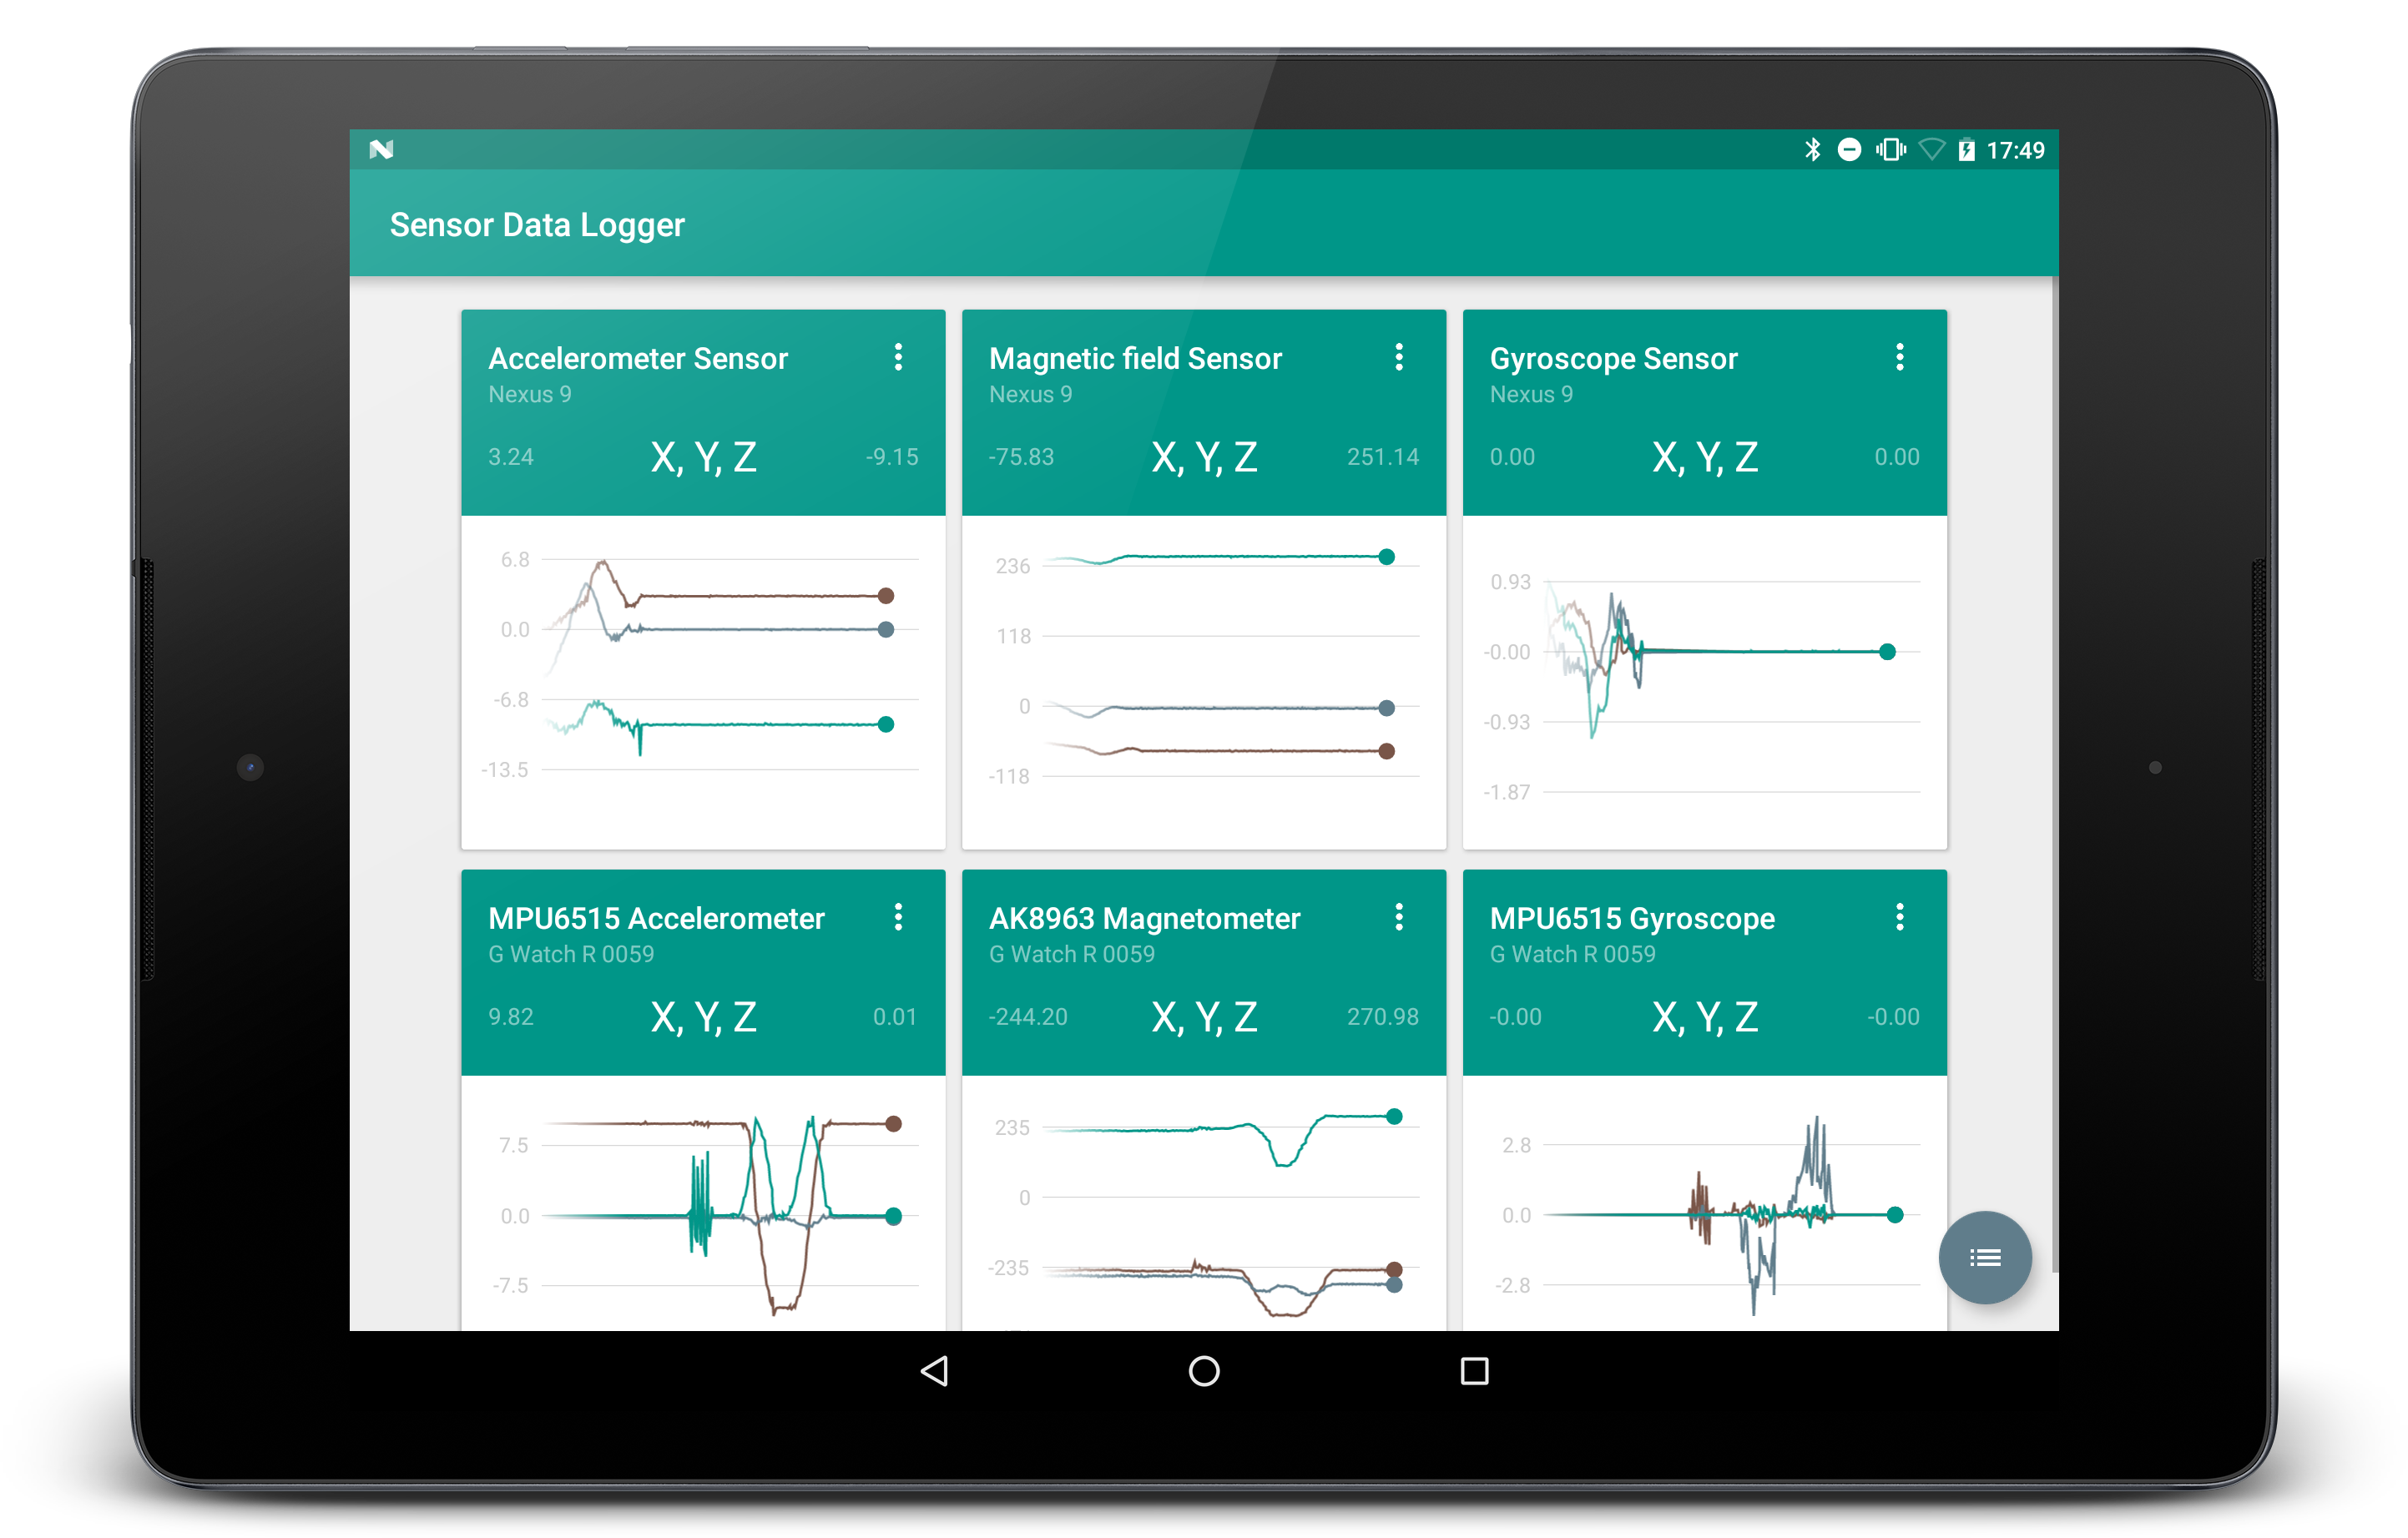
\includegraphics[width=\linewidth]{images/app/charts_landscape_framed.png}
	}
	\caption[Caption for Sensor Data Logger App]{Sensor Data Logger App}
	\label{fig:sensorDataLoggerApp}
\end{figure}

Code samples in the following sections are snippets from this project and can be seen in context in the GitHub repository\footnote{\href{https://github.com/Steppschuh/Sensor-Data-Logger}{https://github.com/Steppschuh/Sensor-Data-Logger}}.

\clearpage

\subsection{Accessing Data}
\label{sec:implementation:accessingdata}

Android provides the |SensorManager|\cite{androiddocs:sensormanager} system service class in order to grant applications access to the device sensors.
The supported sensors can be divided into three categories:

\begin{itemize}[noitemsep]
	\item \textbf{Environmantal sensors} (thermometers, barometers and photometers)
	\item \textbf{Motion sensors} (accelerometers, gyroscopes and gravity sensors)
	\item \textbf{Position sensors} (magnetometers and orientation sensors)
\end{itemize}

Not all sensors are hardware components, the so called ``virtual-'' or ``synthetic sensors'' derive their data from one or more hardware-based sensors.
Examples for these virtual sensors are the linear acceleration sensor, which computes its data based on the accelerometer and the gravity sensor.

All sensors can be accessed through the Android sensor framework, which provides classes and interfaces that can be used to figure out which sensors are available on the current device, which capabilities they have and what data they produce.

\subsubsection{Checking Availability}
\label{sec:implementation:checkingavailability}
While most devices have an accelerometer and a magnetometer, only a few have a thermometer.
The availability of sensors can't be guaranteed, it's good practice to check this at runtime:

\begin{lstlisting}[label=getsensormanager]
// get a SensorManager instance
SensorManager sensorManager = (SensorManager) getSystemService(Context.SENSOR_SERVICE);

// get a list of available sensors
List<Sensor> deviceSensors = sensorManager.getSensorList(Sensor.TYPE_ALL);

// check if an accelerometer is available
Sensor accelerometer = sensorManager.getDefaultSensor(Sensor.TYPE_ACCELEROMETER);
if (accelerometer != null) {
	// use accelerometer
} else {
	// perform error handling
}
\end{lstlisting}

If a sensor is available, public methods from the |Sensor|\cite{androiddocs:sensor} class can be used to get detailed information about it.
The name, vendor, version, data range and reporting delay are useful properties, especially because one device can have multiple sensors of the same type.

\subsubsection{Monitoring Data Changes}
\label{sec:implementation:monitoringdatachanges}
In order to get access to the actual data, a |SensorEventListener|\cite{androiddocs:sensoreventlistener} needs to be registered at the |SensorManager| instance. The |SensorEventListener| is an interface which exposes two callback methods:

\begin{lstlisting}[label=registersensoreventlistener]
// create a new SensorEventListener
SensorEventListener listener = new SensorEventListener() {
	@Override
	public void onSensorChanged(SensorEvent event) {
		// sensor reported new data
	}

	@Override
	public void onAccuracyChanged(Sensor sensor, int accuracy) {
		// sensor accuracy changed
	}
};

// specify a reporting delay for the sensor
int delay = SensorManager.SENSOR_DELAY_NORMAL;

// register the listener for the accelerometer
sensorManager.registerListener(listener, accelerometer, delay);
\end{lstlisting}

The |onSensorChanged| method will be called every time the sensor updates its values. The passed |SensorEvent|\cite{androiddocs:sensorevent} holds the sensor, a timestamp, the accuracy and an array of floats containing the actual values.

If the sensor accuracy changes, which often happens when using location sensors, the |onAccuracyChanged| method will be called.
It can be usefull to care about these accuracies, the location optained from the Cell-ID or Wi-Fi might be more accurate than the latest GPS coordinates for example.
In other cases sensors might need a few seconds to calibrate, like the magnetometer.

When registering a |SensorEventListener|, a delay in microseconds is also passed to the |SensorManager|.
It's worth to notice that this value is more like a suggestion, as other applications and the system can alter it.
Because the reporting delay can impact the battery life of the device, some manufacturers will lower the reporting interval when the device is idle or the display is turned off.

\subsubsection{Monitoring Lifecycle Changes}
\label{sec:implementation:monitoringlifecyclechanges}
Once a |SensorEventListener| is registered, the system will keep the requested sensor active and continue to report data, even if the user leaves the application.
Hence, one should always unregister listeners as soon as possible in order to prevent battery drain:

\begin{lstlisting}[label=basicactivity]
public class SensorActivity extends Activity implements SensorEventListener {
	private SensorManager sensorManager;
	private Sensor accelerometer;

	@Override
	public final void onCreate(Bundle savedInstanceState) {
		super.onCreate(savedInstanceState);
		setContentView(R.layout.main);
		sensorManager = (SensorManager) getSystemService(Context.SENSOR_SERVICE);
		accelerometer = sensorManager.getDefaultSensor(Sensor.TYPE_ACCELEROMETER);
	}

	@Override
	protected void onResume() {
		super.onResume();
		sensorManager.registerListener(this, accelerometer, SensorManager.SENSOR_DELAY_NORMAL);
	}

	@Override
	protected void onPause() {
		super.onPause();
		sensorManager.unregisterListener(this);
	}

	@Override
	public final void onSensorChanged(SensorEvent event) {
		StringBuilder log = new StringBuilder("Acceleration:");
		log.append(" X: ").append(String.valueOf(event.values[0]));
		log.append(" Y: ").append(String.valueOf(event.values[1]));
		log.append(" Z: ").append(String.valueOf(event.values[2]));
		System.out.println(log.toString());
	}

	@Override
	public final void onAccuracyChanged(Sensor sensor, int accuracy) {
		// sensor accuracy changed
	}
}
\end{lstlisting}

This very basic example activity would print accelerometer data to the console once deployed.
Keep in mind that it lacks exception handling, as mentioned in \ref{sec:implementation:checkingavailability}.
We presume a basic understanding of how the Android activity\cite{androiddocs:activity} lifecycle\improvement{Explain} works.

\subsection{Persisting Data}
Once a sensor is reporting data, a new |SensorEvent| will be passed to the callback every few milliseconds.
The |values| float array will contain new data, however the system won't allocate a new object for every update in order to improve performance.
Handling these values without knowing about its object identity might cause confusion, as they will be overwritten with every update.
To prevent this, a new float array can be used to hold the event data:

\begin{lstlisting}[label=arraycopy]
@Override
public void onSensorChanged(SensorEvent event) {
	// create a new float array with the same size
	float[] values = new float[event.values.length];

	// copy data from event values
	System.arraycopy(event.values, 0, values, 0, event.values.length);

	// persist values in some way
	persistValues(values);
}
\end{lstlisting}

For our project, we needed to look back at sensor events from the past few seconds in order to detect patterns and to extract features.
We created some helper classes\cite{sensordatalogger:datapackage} that allowed us to wrap sensor event data in POJOs\footnote{Plain old Java objects}, this way they could be persisted in a batch-like structure.

There is a |Data|\cite{sensordatalogger:data} class which can wrap the values of a |SensorEvent|, its source and a timestamp.
This is necessary because the |SensorEvent| holds references to objects that aren't required multiple times and because there's no public constructor available.

The |DataBatch|\cite{sensordatalogger:databatch} class holds and manages a list of |Data| objects.
It has a customizable capacity, one can add or remove |Data| and it will automatically remove old |Data| if the capacity has been reached.
It also provides some convenience methods, for example to get |Data| from within a given time range.
The following code would fill up a |DataBatch| with event data for each requested sensor type:

\begin{lstlisting}[label=datahelperclasses]
private Map<Integer, DataBatch> sensorDataBatches = new HashMap<>();

@Override
public void onSensorChanged(SensorEvent event) {
	float[] values = new float[event.values.length];
	System.arraycopy(event.values, 0, values, 0, event.values.length);

	// create a new Data object
	Data data = new Data(values);

	// get a previously initialized DataBatch
	DataBatch dataBatch = getDataBatch(event.sensor.getType());

	// add the new data
	dataBatch.addData(data);
}

public DataBatch getDataBatch(int sensorType) {
	DataBatch dataBatch = sensorDataBatches.get(sensorType);
	if (dataBatch == null) {
		dataBatch = new DataBatch(sensorType);
		sensorDataBatches.put(sensorType, dataBatch);
	}
	return dataBatch;
}
\end{lstlisting}

\subsection{Serializing Data}
\label{sec:implementation:serializingdata}

At some point, we have to convert the persisted data into byte arrays.
We need to serialize objects in order to transfer it to another device or to write it into a file.

The most straightforward solution is using JSON\footnote{JavaScript Object Notation}, which is a common data-interchange format.
It is easy to read for humans and easy to parse for software, which is why we decided to use this format.
Fortunately, POJOs can be directly mapped to JSON name-value pairs.
Existing libraries like gson\footnote{https://github.com/google/gson} or jackson\footnote{https://github.com/FasterXML/jackson} are very well known and provide interfaces that make JSON handling very uncomplicated.

The |DataRequestResponse|\cite{sensordatalogger:datarequestresponse} class for example holds a list of |DataBatches| and is responsible for exchaning sensor data with the connected mobile device.
For convenience, all classes that we transfer implement methods that can be used for JSON serialization and deserialization.

\begin{lstlisting}[label=serialization]
@JsonIgnore
public String toJson() {
	String jsonData = null;
	try {
		ObjectMapper mapper = new ObjectMapper();
		mapper.enable(SerializationFeature.INDENT_OUTPUT);
		mapper.disable(SerializationFeature.FAIL_ON_EMPTY_BEANS);
		jsonData = mapper.writeValueAsString(this);
	} catch (Exception ex) {
		ex.printStackTrace();
	}
	return jsonData;
}

public static DataRequestResponse fromJson(String json) {
	DataRequestResponse dataRequestResponse = null;
	try {
		ObjectMapper mapper = new ObjectMapper();
		mapper.disable(SerializationFeature.FAIL_ON_EMPTY_BEANS);
		dataRequestResponse = mapper.readValue(json, DataRequestResponse.class);
	} catch (Exception ex) {
		ex.printStackTrace();
	}
	return dataRequestResponse;
}
\end{lstlisting}

This code block is part of the |DataRequestResponse| class.
The |toJson()| method writes the current object state into a JSON string, while |fromJson(String json)| creates a new |DataRequestResponse| object from a given JSON string.
The JSON string can be converted to a byte array, which can be transferred as described in section \ref{sec:implementation:transferringdata}.
It is crucial that the same character encoding is used, we stick with UTF-8.

\subsection{Transferring Data}
\label{sec:implementation:transferringdata}
Actually using the sensor event data requires transferring it to a device with sufficient processing power.

\subsubsection{General Approach}
In a world where the IoT\footnote{Internet of Things} is a big topic, data is usually uploaded to the cloud and processed on powerfull servers.
Although one could do that from a mobile device, this approach would produce a huge amount of traffic and ultimately lead to privacy concerns.

\begin{figure}[H]
	\centering
	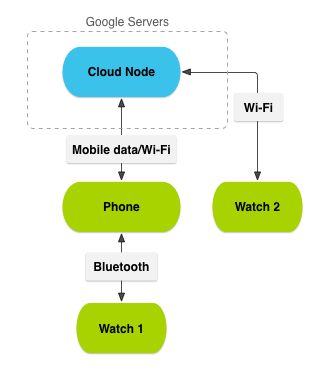
\includegraphics[width=0.5\textwidth]{images/wear_cloud_node.png}
	\caption[Caption for wear_cloud_node]{Sample network with mobile and wearable nodes\footnotemark}
	\label{fig:nodeNetwork}
\end{figure}
\footnotetext{https://developer.android.com/training/wearables/data-layer/}

The setup that this work is about could be seen as a peer to peer network between a mobile device and multiple wearables.
Because the devices are connected with each other, there's no need to detour data through the internet.
By default, wearables are connected via Bluetooth with a mobile device.
On the Android platform, this connection can be accessed through the |WearableApi|\cite{androiddocs:wearable}.

\clearpage

\subsubsection{The Wearable Data Layer}

The Data Layer API is part of of the Google Play Services.
It contains the only APIs that should be used to set up a communication channel between a mobile device and wearable devices. 
Custom, low-level socket implementations are not recommended.

As shown in figure \ref{fig:nodeNetwork}, the Data Layer API can handle multiple nodes at once.
We are particularly interested in the Bluetooth channel, but we don't have to care about the connection because this is handled by the Play Services for us.
The API can be reached using an instance of the |GoogleApiClient|\cite{androiddocs:googleapiclient}.
Because some Play Services may not be available on every device, the |GoogleApiClient| needs to be setup first:

\begin{lstlisting}[label=googleapiclient]
GoogleApiClient googleApiClient = new GoogleApiClient.Builder(context)
		.addConnectionCallbacks(new ConnectionCallbacks() {
			@Override
			public void onConnected(Bundle connectionHint) {
				// start using the Data Layer API
			}
			@Override
			public void onConnectionSuspended(int cause) {
				// something interrupted the connection
			}
		})
		.addOnConnectionFailedListener(new OnConnectionFailedListener() {
			@Override
			public void onConnectionFailed(ConnectionResult result) {
				// API might not be available
			}
		})
		.addApi(Wearable.API)
		.build();
\end{lstlisting}

This code block would initialize a |GoogleApiClient| instance.
However, |addApi(Wearable.API)| would cause a call to |onConnectionFailed| if the device it runs on doesn't have the Android Wear app\footnote{https://play.google.com/store/apps/details?id=com.google.android.wearable.app} installed.
This app is required because it handles the connection and synchronization of wearables.
For more gracefull error handling, |addApiIfAvailable(Wearable.API)| might be the more appropriate solution.

\subsubsection{The Message API}

There are multiple ways of exchanging data between nodes using the Data Layer API.
While the |DataApi|\cite{androiddocs:dataapi} can be used to synchronize larger binary blobs (|Assets|\cite{androiddocs:asset}) accross the wearable network, the |MessageApi|\cite{androiddocs:messageapi} is more suitable for exchanging smaller amounts of data.
A message consists of the following items:
\begin{itemize}[noitemsep]
	\item \textbf{Path}:
	A string that uniquely identifies the message action. 
	\item \textbf{Payload}:
	An optional byte array.
\end{itemize}
Payloads are not required by default because messages are a one-way communication mechanism, often used to only trigger RPCs\footnote{Remote procedure calls}. We use this to pass a serialized |DataRequest|\cite{sensordatalogger:datarequest} or |DataRequestResponse|\cite{sensordatalogger:datarequestresponse}.

\subsubsection{Sending Messages}
\label{sec:implementation:transferringdata:send}

In order to send a message to a connected wearable, the |Node|\cite{androiddocs:node} representation of that device is required.
We can use the |NodeApi|\cite{androiddocs:nodeapi} to query connected nodes:

\begin{lstlisting}[label=nodes]
// a list that holds available nodes
private List<Node> nearbyNodes;

private void updateNearbyNodes() {
	Wearable.NodeApi.getConnectedNodes(googleApiClient)
			.setResultCallback(new ResultCallback<NodeApi.GetConnectedNodesResult>() {
				@Override
				public void onResult(NodeApi.GetConnectedNodesResult nodes) {
					nearbyNodes = new ArrayList<Node>();

					// add all nearby nodes to the list
					for (Node node: nodes.getNodes()) {
						if (node.isNearby()) {
							nearbyNodes.add(node);
						}
					}
				}
			});
}
\end{lstlisting}

The |nearbyNodes| list now contains all currently connected wearables.
We can get a display name and an id for each node, which we need to select our message target.
For simplicity, the following code block sends a message to all nearby nodes:

\begin{lstlisting}[label=sendmessage]
private void startRequestingSensorData() {
	// send a request message to all nodes
	sendMessageToNearbyNodes("/start_requesting_sensor_data", null);
}

private void sendMessageToNearbyNodes(String path, byte[] payload) {
	for (Node node: nearbyNodes) {
		sendMessageToNode(node.getId(), path, payload);
	}
}

private void sendMessageToNode(String nodeId, String path, byte[] payload) {
	Wearable.MessageApi.sendMessage(googleApiClient, nodeId, path, payload)
			.setResultCallback(new ResultCallback() {
				@Override
				public void onResult(SendMessageResult sendMessageResult) {
					if (!sendMessageResult.getStatus().isSuccess()) {
						// perform exception handling
					}
				}
			});
}
\end{lstlisting}

Note that we can pass |null| as a payload if no data is required.
Instead of null, a serialized |DataRequest| object could be passed.
The receiving nodes could deserialize it to find out which sensors are requested or at which interval they should report updates.

\subsubsection{Receiving Messages}
\label{sec:implementation:transferringdata:receive}

Apps running on the wearables need to implement the |MessageListener|\cite{androiddocs:messagelistener} interface in order to get notified about incoming messages. These listeners have to be registered using the |MessageApi.addListener()| function.

\begin{lstlisting}[label=receivemessage]
@Override
public void onMessageReceived(MessageEvent messageEvent) {
    if (messageEvent.getPath().equals("/start_requesting_sensor_data")) {
        // get the message payload
        byte[] payload = messageEvent.getData();

        // process the request
        startTransferringSensorData();
    }
}
\end{lstlisting}

Obviously, message paths should be static and final constants defined in a shared module that the mobile and wearable app package have access to. In our implementation, the payload would be a serialized |DataRequest|.

\improvement{Explain ChannelApi}

\subsection{Putting it all together}
asdf

\improvement{Change section title}

\clearpage
	\section{Evaluation}
\label{sec:evaluation}

In order to measure how performant different implementations are, we created different benchmarks.
These helped us to evaluate which parts of our solution require optimization.
Each benchmark contains the average result of 500 consecutive measurements and has been validated multiple times.

\subsection{Setup}
For the benchmarks, we created a |TimeTracker|\cite{sensordatalogger:timetracker} that is capable of measuring the delay in nanoseconds between events. It also provides convenience functions for merging repetitive measurements to avoid round-off errors.

We measured on our test devices, a Nexus 9 tablet (released November 2014, SDK 24) and a LG G Watch R (released October 2014, SDK 23). Both ran the latest Android version and are a good representation for currently available high-end devices.
The devices were placed next to each other on a table, with quite a lot of other electronic devices nearby.
We also altered the distance between the devices but figured out that it had no significant impact on the measurements.

\subsection{Data Transmission Delay}
The most important performance indicator is the time it takes between these events: \textit{A sensor has updated values} (on the wearable device) and \textit{Updated sensor values have been received} (on the mobile device). For this benchmark, the measured operations include:

\begin{itemize}[noitemsep]
    \item Creating |DataBatches|\cite{sensordatalogger:databatch} with the latest sensor data (wearable)
    \item Serializing a |DataRequestResponse|\cite{sensordatalogger:datarequestresponse} containing that data (wearable)
    \item Transferring the data using the |MessageApi|\cite{androiddocs:messageapi} (wearable \& mobile)
    \item Deserializing the |DataRequestResponse| (mobile)
\end{itemize}

In order to reduce the serialization overhead, we collect sensor data in |DataBatches|\cite{sensordatalogger:databatch} before transferring it to a mobile device.
This approach drastically improves the \textit{delay per sent byte} ratio, because we have to serialize and deserialize less messages and less meta data.
However, it also delays the data depending on the batch capacity.
Just like buffering a stream, this is a trade-off between being less efficient or being less real-time.

For the measurements in table \ref{table:benchmark:transmissiondelay:50ms}, we batched sensor data from the accelerometer for \textbf{50 milliseconds} before transferring it while altering the sensor delay:

\begin{table}[H]
    \begin{tabular}{rrrl}
        delay in ns       & bytes             & delay / bytes                   & comment \\ \hline

        1,266,250,000     & 200               & \textasciitilde6,331,250        & \textasciitilde1 update (|SENSOR_DELAY_NORMAL|) \\
        1,271,160,000     & 482               & \textasciitilde2,637,261        & \textasciitilde2 updates (|SENSOR_DELAY_UI|) \\
        1,285,510,000     & 1,056             & \textasciitilde1,217,339        & \textasciitilde6 updates (|SENSOR_DELAY_GAME|) \\
        1,306,400,000     & 3,599             & \textasciitilde362,989          & \textasciitilde24 updates (|SENSOR_DELAY_FASTEST|) \\
    \end{tabular}
    \caption{Transmission delay, 50ms batches}
    \label{table:benchmark:transmissiondelay:50ms}
\end{table}

When using |SENSOR_DELAY_NORMAL|, the sensor reports only about one update during the batching duration.
This basically results in no improvement at all because we still have to deal with the serialization overhead for each update.
By collecting more updates in the same time frame (in this case by switching to |SENSOR_DELAY_FASTEST|), we were able to boost the efficency by 94.3\% while only raising the delay by 3.2\%.

We wanted to improve even further and increased the batching duration to \textbf{500 milliseconds}, as measured in table \ref{table:benchmark:transmissiondelay:500ms}:

\begin{table}[H]
    \begin{tabular}{rrrl}
        delay in ns       & bytes             & delay / bytes                   & comment \\ \hline

        1,329,120,000     & 625               & \textasciitilde2,126,592        & \textasciitilde3 updates (|SENSOR_DELAY_NORMAL|) \\
        1,331,970,000     & 1,340             & \textasciitilde994,007          & \textasciitilde8 updates (|SENSOR_DELAY_UI|) \\
        1,373,370,000     & 8,262             & \textasciitilde166,227          & \textasciitilde28 updates (|SENSOR_DELAY_GAME|) \\
        1,412,810,000     & 16,951            & \textasciitilde83,346           & \textasciitilde118 updates (|SENSOR_DELAY_FASTEST|) \\
    \end{tabular}
    \caption{Transmission delay, 500ms batches}
    \label{table:benchmark:transmissiondelay:500ms}
\end{table}

Increasing the duration resulted in more updates per transferred |DataRequestResponse|\cite{sensordatalogger:datarequestresponse}.
Compared to the first measurement in table \ref{table:benchmark:transmissiondelay:50ms}, we were able to transfer 84 times more bytes at the cost of only 147 milliseconds.

For some use cases, less frequent data might be sufficient. Instead of altering the reporting delay of the sensor, we can also sent data from multiple sensors simultaneously. Table \ref{table:benchmark:transmissiondelay:multiple} shows how \textbf{multiple, 3-dimensional sensors} perform:

\begin{table}[H]
    \begin{tabular}{rrrl}
        delay in ns       & bytes             & delay / bytes                   & comment \\ \hline

        1,452,400,000     & 16,690            & \textasciitilde87,022           & \textasciitilde116 updates,  1 sensor \\
        1,489,100,000     & 22,819            & \textasciitilde65,257           & \textasciitilde246 updates,  2 sensors \\
        1,752,420,000     & 60,679            & \textasciitilde28,880           & \textasciitilde512 updates,  4 sensors \\
        2,842,640,000     & 177,495           & \textasciitilde16,015           & \textasciitilde1504 updates, 8 sensors \\
    \end{tabular}
    \caption{Transmission delay, multiple sensors}
    \label{table:benchmark:transmissiondelay:multiple}
\end{table}

Keeping in mind that this transfer is performed multiple hundreds or thousands times, these efficency improvements sum up and save a lot of computing and battery power on both devices.

\subsection{Serialization}
As mentioned before, serialization and deserialization are responsible for a large part of the processing time.
It is crucial that this part is optimized, that's why we opted for utilizing established libraries.
Namely, we decided to use jackson\footnote{https://github.com/FasterXML/jackson} because of its performance advantage compared to other well known libraries like gson\footnote{https://github.com/google/gson}.

There are benchmarks available that compare these JSON libraries, which is why we won't present new measurements here.
The key take-away is that jackson is faster in handling larger files, while gson should be used for smaller files\footnote{http://blog.takipi.com/the-ultimate-json-library-json-simple-vs-gson-vs-jackson-vs-json/}.

\subsection{Data Rate}
asdf

\subsection{Battery Impact}
Of course the heavy usage of the Bluetooth sensor and processing power brings along the cost of reduced battery life.
Because battery power is very limited on mobile devices, we also benchmarked the power consumption of our app and the related system processes.
Each measurement contains the consumed milliamp hours (mAh) during a one hour period.

We observed the processes with the largest battery impact, the following tables contain the consumption of:

\begin{itemize}[noitemsep]
    \item \textbf{Total}: The overall device
    \item \textbf{System}: Android System related packages
    \item \textbf{OS}: Android OS related packages
    \item \textbf{BT}: Bluetooth sensor
    \item \textbf{Screen}: Device display
    \item \textbf{App}: Sensor Data Logger package
\end{itemize}

To get some reference values, we observed the idle state first.
Mobile and wearable device are connected and only casually used to reply to messages:

\begin{table}[H]
    \centering
    \begin{tabular}{rrrrrr}
        Total    & System   & OS       & BT       & Screen   & App  \\ \hline

        163      & 27       & 20       & 13       & 32       & 0    \\
        173      & 30       & 22       & 15       & 52       & 0    \\
        173      & 34       & 19       & 13       & 39       & 0    \\
        160      & 27       & 25       & 13       & 40       & 0    \\
    \end{tabular}
    \caption{Battery impact, idle}
    \label{table:benchmark:battery:idle}
\end{table}

We measured an average total battery drain of 167 mAh per hour.
Assuming that the average battery capacity of currently available smartphones is \textasciitilde2500 mAh, this is equivalent to 6.68\% of battery life.

The Bluetooth consumption is noticeable because the wearable is connected to the phone and synchronizing notifications, although it is not streaming sensor data.

To benchmark how the app influences the power consumption, we requested 3-dimensional data from the accelerometer and gravity sensor with |SENSOR_DELAY_FASTEST| every 50 ms. The measured operations include:

\begin{itemize}[noitemsep]
    \item Transferring the data using the |MessageApi| (wearable \& mobile)
    \item Deserializing the |DataRequestResponse| (mobile)
    \item Processing the |DataBatches| (mobile)
    \item Rendering the |Data|\cite{sensordatalogger:data} (mobile)
\end{itemize}

\begin{table}[H]
    \centering
    \begin{tabular}{rrrrrr}
        Total    & System   & OS       & BT       & Screen   & App  \\ \hline

        615      & 65       & 97       & 32       & 162      & 226  \\
        580      & 59       & 99       & 32       & 148      & 239  \\
        593      & 67       & 91       & 34       & 161      & 226  \\
        630      & 71       & 103      & 32       & 151      & 219  \\
    \end{tabular}
    \caption{Battery impact, with processing and rendering}
    \label{table:benchmark:battery:screen}
\end{table}

The average total battery drain has increased by a factor of 3.6 to 605 mAh per hour.
One can see that all observed processes consumed at least twice as much battery.
As expected, the app itself is responsible for the largest battery impact with an average of 228 mAh.

However, a huge amount of power was required for the processing and rendering steps, which may be not required in every use case.
Also, we forced the screen to be turned on at 20\% brightness, which can also be avoided.

For the following measurements we excluded the processing and rendering steps and did not force the screen to be on:

\begin{table}[H]
    \centering
    \begin{tabular}{rrrrrr}
        Total    & System   & OS       & BT       & Screen   & App  \\ \hline

        331      & 60       & 88       & 34       & 41       & 57   \\
        318      & 59       & 92       & 30       & 38       & 64   \\
        330      & 53       & 94       & 33       & 32       & 63   \\
        325      & 57       & 92       & 33       & 40       & 59   \\
    \end{tabular}
    \caption{Battery impact, without processing and rendering}
    \label{table:benchmark:battery:noscreen}
\end{table}

Although all processes still require more power compared to the idle state, the average total battery drain has only increased by a factor of 1.9 to 326 mAh per hour.
The |Data| processing and rendering steps were responsible for 73\% of the apps battery drain.

\improvement{Add visualization}

\clearpage
	\section{Future Work}
\label{sec:futurework}

\subsection{Open Research Questions}
What could other researches work on?

\subsection{Extensions}

\subsubsection{Channel API}
In our implementation, we utilized the |MessageApi|\cite{androiddocs:messageapi} because it is recommended for smaller messages.
We also used it for other project related purposes, so we sticked to it for consistency.
However, we figured out that there might be an even more performant solution:

The |ChannelApi|\cite{androiddocs:channelapi} is also part of the |WearableApi|\cite{androiddocs:wearable}, accessible through the |GoogleApiClient|\cite{androiddocs:googleapiclient}.
It should be used to transfer large files, just like the already mentioned |DataApi|\cite{androiddocs:dataapi}.
In contrast to the |DataApi|, it doesn't synchronize |Assets|\cite{androiddocs:asset} across the devices.
Instead, it creates a bidirectional channel that the sending and receiving node may read or write to.
Data can be exchanged using byte streams, which makes the |ChannelApi| very suitable for transferring streamed content like music - or even sensor data.

Unfortunately we weren't able to evaluate whether implementing the |ChannelApi| would increase our performance yet.

\subsubsection{Compression}
In order to decrease the amount of data transferred with each |DataRequestResponse|\cite{sensordatalogger:datarequestresponse}, we can try to reduce the overhead created by meta data.
This overhead can only be reduced to a certain amount, though.

Each sensor data update is an array of values, and can have up to 9 dimensions (depending on the sensor).
Each dimension holds a single-precision 32-bit IEEE 754 floating point.
In our use case, we didn't need values with that high precision.
Instead, rounded values would be sufficient for our algorithms.

By switching the data type of our data arrays from floats to shorts (16-bit signed two's complement integers), we could save about 50\% of transferred bytes. However, it still has to be evaluated whether the loss of precision and the processing power required for converting the data justifies this saving.

\clearpage
	\section{Conclusion}
\label{sec:conclusion}

To achieve our project goal of a seamless authentication using nothing but the sensors from a user's devices, we need to transfer huge amounts of data every second.
Our solution provides a performant jet battery friendly way of exchanging messages with data payloads between wearables and mobile devices.
It allowed us to develop a product that fulfilled all our project requirements.

We also implemented our solution in an open source app\footnote{\href{https://github.com/Steppschuh/Sensor-Data-Logger}{https://github.com/Steppschuh/Sensor-Data-Logger}} that is available for free through the Google Play Store\footnote{\href{https://play.google.com/store/apps/details?id=net.steppschuh.sensordatalogger}{https://play.google.com/store/apps/details?id=net.steppschuh.sensordatalogger}}.
It is capable of visualizing sensor data from the current mobile or a connected wearable device in real-time.
This app can be used as a reference for related research and for demonstration purposes.

\clearpage
	
	%%% Bibliography
	%\bibliographystyle{babunsrt3-fl}
	\addcontentsline{toc}{section}{Bibliography}
	\bibliographystyle{babunsrt-fl}
	\bibliography{projektbib}
	\clearpage	
	
	%%%% Appendix
	\appendix
\section{Appendix}
\label{sec:appendix}

Lorem ipsum dolor sit amet, consectetur adipiscing elit. In erat mauris, faucibus quis pharetra sit amet, pretium ac libero. Etiam vehicula eleifend bibendum. Morbi gravida metus ut sapien condimentum sodales mollis augue sodales. Vestibulum quis quam at sem placerat aliquet. Curabitur a felis at sapien ullamcorper fermentum. Mauris molestie arcu et lectus iaculis sit amet eleifend eros posuere. Fusce nec porta orci.

Integer vitae neque odio, a sollicitudin lorem. Aenean orci mauris, tristique luctus fermentum eu, feugiat vel massa. Fusce sem sem, egestas nec vulputate vel, pretium sit amet mi. Fusce ut nisl id risus facilisis euismod. Curabitur et elementum purus. Duis tincidunt fringilla eleifend. Morbi id lorem eu ante adipiscing feugiat. Sed congue erat in enim eleifend dignissim at in nisl. Donec tortor mauris, mollis vel pretium vitae, lacinia nec sapien. Donec erat neque, ullamcorper tincidunt iaculis sit amet, pharetra bibendum ipsum. Nunc mattis risus ac ante consequat nec pulvinar neque molestie. Etiam interdum nunc at metus lacinia non varius erat dignissim. Integer elementum, felis id facilisis vulputate, ipsum tellus venenatis dui, at blandit nibh massa in dolor. Cras a ultricies sapien. Vivamus adipiscing feugiat pharetra.
\clearpage
	
	%%% TODOs
	%\todo[inline]{The original todo note withouth changed colours.\newline Here's another line.}
	%\lipsum[1]\unsure{Is this correct?}\unsure{I'm unsure about also!}
	%\lipsum[1]\change{Transate abstract}
	%\lipsum[1]\info{This can help me in chapter seven!}
	%\lipsum[1]\improvement{This really needs to be improved!\newline\newline What was I thinking?!}
	%\thiswillnotshow{This is hidden since option `disable' is chosen!}
	%\improvement[inline]{The following section needs to be rewritten!}
	\listoftodos[Notes]
	
\end{document}